\section{Introduction}
\begin{frame}{}
    \LARGE Natural Language Processing: \textbf{Introduction}
\end{frame}

\begin{frame}[allowframebreaks]{NLP - Introduction}
    \large \textbf{What is NLP?}
    \begin{itemize}
        \item Study of computational approaches to processing natural languages.
        \item Processing includes:
            \begin{itemize}
                \item Acquiring language data
                \item Representing information
                \item Storing text and speech
                \item Understanding meaning
                \item Characterizing language patterns
                \item Generating new language
            \end{itemize}
        \item Natural languages refer to human languages.
    \end{itemize}
\framebreak
    \begin{figure}
        \centering
        \fetchconvertimage{https://www.qtravel.ai/wp-content/uploads/2023/12/what-is-natual-language-processsing-1024x884.png}{images/nlp-intro/nlp-about.png}{width=\textwidth,height=0.9\textheight,keepaspectratio}
    \end{figure}
\framebreak
    {\large \textbf{NLP = Computer Science + Linguistics + AI}}

    \begin{itemize}
        \item \textbf{Deals with:}
        \begin{itemize}
            \item Language understanding (input)
            \item Language generation (output)
            \item Language translation
            \item Information extraction
        \end{itemize}
        \item \textbf{Subfields:}
        \begin{itemize}
            \item Syntax
            \item Semantics
            \item Pragmatics
            \item Discourse
        \end{itemize}
    \end{itemize}
\end{frame}

\begin{frame}[allowframebreaks]{Goal}
    \begin{figure}
        \centering
        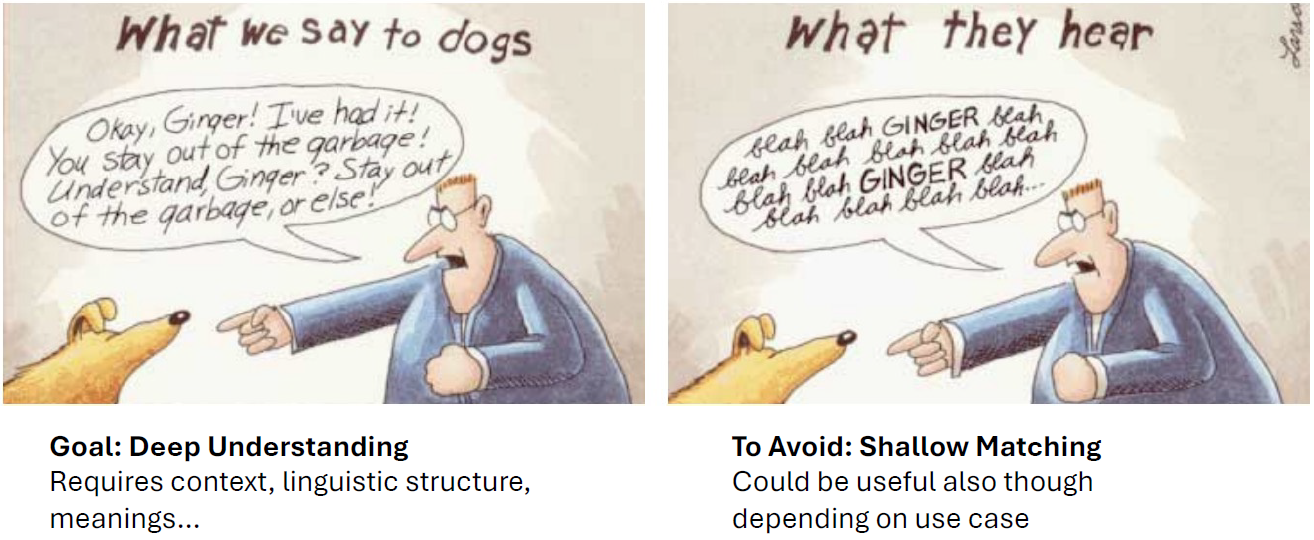
\includegraphics[width=\textwidth,height=0.9\textheight,keepaspectratio]{images/nlp-intro/goal.png}
    \end{figure}
\framebreak
    \large \textbf{Goal of NLP:}
    \begin{itemize}
        \setlength{\itemsep}{1em}
        \item Enable machines to understand and generate human language.
        \item Facilitate human-computer interaction through natural language.
        \item Develop systems that can process and analyze large amounts of text data.
    \end{itemize}
\end{frame}

\begin{frame}[allowframebreaks]{NLP Pipeline}
    \begin{itemize}
        \item \textbf{Text Preprocessing}
        \vspace{-0.5em}
        \begin{itemize}
            \item Cleaning and preparing raw text for analysis.
        \end{itemize}
        \item \textbf{Tokenization}
        \vspace{-0.5em}
        \begin{itemize}
            \item Splitting text into words, sentences, or other meaningful units.
        \end{itemize}
        \item \textbf{POS Tagging}
        \vspace{-0.5em}
        \begin{itemize}
            
            \item Assigning parts of speech (noun, verb, etc.) to each token.
        \end{itemize}
        \item \textbf{Parsing}
        \vspace{-0.5em}
        \begin{itemize}
            
            \item Analyzing grammatical structure of sentences.
        \end{itemize}
        \item \textbf{Named Entity Recognition (NER)}
        \vspace{-0.5em}
        \begin{itemize}
            
            \item Identifying entities such as people, organizations, locations.
        \end{itemize}
        \item \textbf{Sentiment Analysis / Classification}
        \vspace{-0.5em}
        \begin{itemize}
            
            \item Determining sentiment or categorizing text.
        \end{itemize}
        \item \textbf{Language Modeling}
        \vspace{-0.5em}
        \begin{itemize}
            
            \item Predicting the next word or sequence in text.
        \end{itemize}
    \end{itemize}
\end{frame}

\begin{frame}[allowframebreaks]{Text Data is Superficial}
    \large
    \begin{itemize}
        \item An iceberg is a large piece of freshwater ice that has broken off from a snow-formed glacier or ice shelf and is floating in open water.
    \end{itemize}
    \vspace{1em}
    \begin{figure}
        \centering
        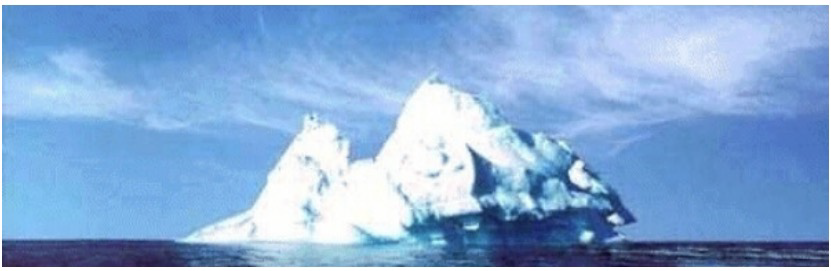
\includegraphics[width=\textwidth,height=0.7\textheight,keepaspectratio]{images/nlp-intro/iceberg-1.png}
    \end{figure}    
\end{frame}

\begin{frame}[allowframebreaks]{Text Data is Superficial}
    \large
    \begin{columns}
        \begin{column}{0.5\textwidth}
            \begin{itemize}
                \item An iceberg is a large piece of freshwater ice that has broken off from a snow-formed glacier or ice shelf and is floating in open water.
            \end{itemize}
        \end{column}
        \begin{column}{0.5\textwidth}
            \begin{figure}
                \centering
                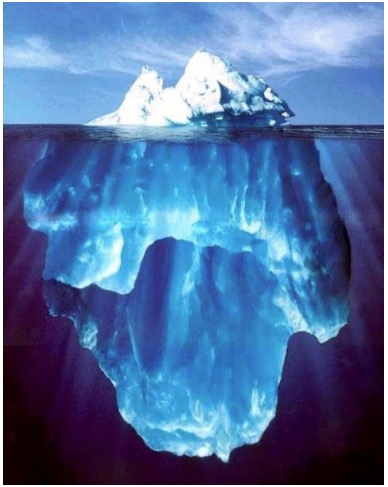
\includegraphics[width=\textwidth,height=0.9\textheight,keepaspectratio]{images/nlp-intro/iceberg-2.png}
            \end{figure}
        \end{column}
    \end{columns}
\end{frame}    

\begin{frame}[allowframebreaks]{NLP Basics – What It’s All About}
    \vspace{-1em}
    Teaching machines to \textbf{understand and generate human language}
    \begin{itemize}
        \item \textbf{Text preprocessing}: \\
        {\small Cleaning and preparing raw text data (removing noise, tokenization, normalization).}
        \item \textbf{Understanding meaning}: \\
        {\small Extracting meaning from text using techniques like part-of-speech tagging, named entity recognition, and sentiment analysis.}
        \item \textbf{Language modeling}: \\
        {\small Building models that can predict or generate text, such as autocomplete or next-word prediction.}
        \item \textbf{Translation, summarization, etc.}: \\
        {\small Enabling applications like machine translation, text summarization, question answering, and more.}
    \end{itemize}

    \textcolor{blue}{Text data is everywhere: tweets, reviews, articles, chats! NLP helps us make sense of this vast information.}

\end{frame}

\begin{frame}[allowframebreaks]{Core NLP Tasks}
\begin{table}[ht]
    \centering
    \renewcommand{\arraystretch}{1.8} % Increased row spacing
    \begin{tabular}{@{} p{0.3\textwidth} p{0.3\textwidth} p{0.4\textwidth} @{}}
        \toprule
        \textbf{Task} & \textbf{What It Does} & \textbf{Example} \\
        \midrule
        \hline % Horizontal line after header row
        \textbf{Tokenization} & Split text into words & \texttt{"I love NLP"} $\rightarrow$ \texttt{["I", "love", "NLP"]} \\
        \textbf{POS Tagging} & Label grammar tags & \texttt{"Dogs bark"} $\rightarrow$ [Noun, Verb] \\
        \textbf{Named Entity Recognition} & Find names, places, etc. & \texttt{"Christopher Nolan lives in Los Angeles"} \\
        \textbf{Sentiment Analysis} & Detect mood & \texttt{"This movie was amazing!"} $\rightarrow$ Positive \\
        \textbf{Machine Translation} & Language to language & English $\rightarrow$ French \\
        \bottomrule
    \end{tabular}
\end{table}
\end{frame}


\begin{frame}{Text Preprocessing}
    \begin{itemize}
        \item \textbf{Lowercase everything}: \\
        {\small Example: \texttt{"NLP"} $\rightarrow$ \texttt{"nlp"}}
        \item \textbf{Removing stop words}: \\
        {\small Eliminate common words that carry little meaning (e.g., "is", "the", "and") to focus on important content.}
        \item \textbf{Stemming/Lemmatization}: \\
        {\small Reduce words to their root or base form. \\
        Example: \texttt{"running"} $\rightarrow$ \texttt{"run"}}
        \item \textbf{Vectorization}: \\
        {\small Transform words or documents into numerical representations for machine learning models:
        \begin{itemize}
            \item \textbf{Bag of Words}: Counts word occurrences in a document.
            \item \textbf{TF-IDF (Term Frequency-Inverse Document Frequency)}: Weighs words by importance across documents.
            \item \textbf{Word2Vec}: Learns dense vector representations capturing word meaning and context.
        \end{itemize}}
    \end{itemize}
\end{frame}

\begin{frame}[allowframebreaks]{Corpora}
    % \large
    \begin{columns}
        \begin{column}{0.4\textwidth}
            \begin{figure}
                \centering
                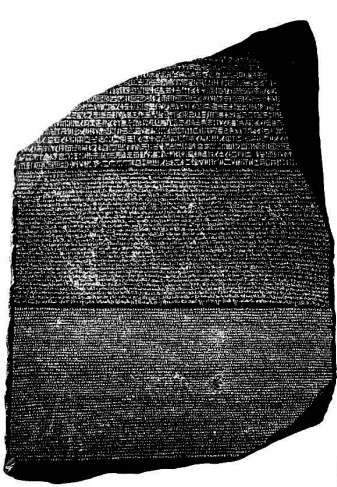
\includegraphics[width=\textwidth,height=0.9\textheight,keepaspectratio]{images/nlp-intro/corpora.png}
            \end{figure}
        \end{column}
        \begin{column}{0.6\textwidth}
            \textbf{What is a corpus?}
            \begin{itemize}
                \item A corpus is a collection of text.
                \item Often annotated in some way.
                \item Sometimes just lots of text.
                \item \textbf{Balanced corpora:} Usually not possible in practice.
                \item \textbf{Examples:}
                \begin{itemize}
                    \item Newswire collections: 500M+ words
                    \item Brown corpus: 1M words of tagged ``balanced'' text
                    \item Penn Treebank: 1M words of parsed WSJ
                    \item Canadian Hansards: 10M+ words of aligned French/English sentences
                    \item The Web: billions of words of who knows what
                \end{itemize}
            \end{itemize}
        \end{column}
    \end{columns}
\end{frame}

\begin{frame}{What is Vocabulary in NLP?}
    \begin{itemize}
        \item \textbf{Vocabulary} = All unique words in your dataset
        \item Example: \texttt{"I love NLP and NLP loves me"} $\rightarrow$ \\
        Vocabulary = \{\texttt{"I"}, \texttt{"love"}, \texttt{"NLP"}, \texttt{"and"}, \texttt{"loves"}, \texttt{"me"}\}
        \item More data = Bigger vocabulary = Harder to process!
    \end{itemize}
    \vspace{1em}
    \textcolor{blue}{\faLightbulbO\enspace Tip: Rare words may not help; common words may not mean much.}
\end{frame}

\begin{frame}{The Problem with Sparse Representations}
    \textbf{Traditional approach: One-hot encoding}
    \begin{itemize}
        \item Example: \texttt{"NLP"} $\rightarrow$ [0, 0, 1, 0, 0, 0, 0\ldots]
    \end{itemize}
    \vspace{1em}
    \textbf{Problem:}
    \begin{itemize}
        \item High-dimensional (thousands of words!)
        \item Sparse (mostly 0s)
        \item No meaning in structure (no relation between \texttt{"king"} and \texttt{"queen"})
        \item \textcolor{red}{\faTimes\enspace Not efficient for learning}
    \end{itemize}
\end{frame}

\begin{frame}{Word Frequencies \& Feature Extraction}
    \textbf{Feature extraction = Turning text into numbers}
    \begin{itemize}
        \item Count how often each word appears (\textbf{Term Frequency})
    \end{itemize}
    \vspace{1em}
    \textbf{Example:}
    \begin{table}[ht]
        \centering
        \renewcommand{\arraystretch}{1.8} % Increased row spacing
        \begin{tabular}{lcc}
            \toprule
            \textbf{Text} & \texttt{"great product"} & \texttt{"bad product"} \\
            \midrule
            Word: \texttt{"great"} & 1 & 0 \\
            Word: \texttt{"bad"} & 0 & 1 \\
            \bottomrule
        \end{tabular}
    \end{table}
    \vspace{0.5em}
    \textcolor{blue}{\faBalanceScale\enspace Use this to find patterns in sentiment, spam, etc.}
\end{frame}

\begin{frame}{Positive \& Negative Frequencies}
    Suppose you're classifying reviews:

    \vspace{0.5em}
    \textbf{Positive Reviews:} \texttt{["amazing", "good", "great"]} \\
    \textbf{Negative Reviews:} \texttt{["bad", "awful", "terrible"]}

    \vspace{1em}
    Count how often each word appears in each class.

    \vspace{1em}
    \textbf{Example table:}
    \begin{table}[ht]
        \centering
        \renewcommand{\arraystretch}{1.5}
        \begin{tabular}{lcc}
            \toprule
            \textbf{Word} & \textbf{Positive Count} & \textbf{Negative Count} \\
            \midrule
            good & 20 & 1 \\
            bad & 1 & 30 \\
            \bottomrule
        \end{tabular}
    \end{table}

    \vspace{0.5em}
    Helps models detect the “tone” (\textbf{sentiment clues}) of new text.
\end{frame}

\begin{frame}{Feature Extraction Techniques}
    \begin{itemize}
        \item \textbf{Bag of Words (BoW)}: Just counts word frequencies in each document.
        \item \textbf{TF-IDF (Term Frequency-Inverse Document Frequency)}: Adjusts for how “unique” or important a word is in a document compared to all documents.
        \begin{itemize}
            \item Words like \texttt{"the"}, \texttt{"is"} are less important.
        \end{itemize}
        \item \textbf{Word Embeddings (later)}: Add meaning and capture relationships between words (e.g., similarity, analogy).
    \end{itemize}
\end{frame}